%%
%% This is file `sample-sigchi.tex',
%% generated with the docstrip utility.
%%
%% The original source files were:
%%
%% samples.dtx  (with options: `sigchi')
%% 
%% IMPORTANT NOTICE:
%% 
%% For the copyright see the source file.
%% 
%% Any modified versions of this file must be renamed
%% with new filenames distinct from sample-sigchi.tex.
%% 
%% For distribution of the original source see the terms
%% for copying and modification in the file samples.dtx.
%% 
%% This generated file may be distributed as long as the
%% original source files, as listed above, are part of the
%% same distribution. (The sources need not necessarily be
%% in the same archive or directory.)
%%
%% The first command in your LaTeX source must be the \documentclass command.

\documentclass[sigchi]{acmart}
\usepackage{float}
\usepackage{caption}
\usepackage{booktabs}
\newcommand{\rpm}{\sbox0{$1$}\sbox2{$\scriptstyle\pm$}
  \raise\dimexpr(\ht0-\ht2)/2\relax\box2 }

%%
%% \BibTeX command to typeset BibTeX logo in the docs
\AtBeginDocument{%
  \providecommand\BibTeX{{%
    \normalfont B\kern-0.5em{\scshape i\kern-0.25em b}\kern-0.8em\TeX}}}

%% Rights management information.  This information is sent to you
%% when you complete the rights form.  These commands have SAMPLE
%% values in them; it is your responsibility as an author to replace
%% the commands and values with those provided to you when you
%% complete the rights form.
\copyrightyear{2019}
\acmYear{2019}

%% These commands are for a PROCEEDINGS abstract or paper.
\acmConference{CPSC 448A}{2018W1}{UBC Vancouver, BC}


%%
%% Submission ID.
%% Use this when submitting an article to a sponsored event. You'll
%% receive a unique submission ID from the organizers
%% of the event, and this ID should be used as the parameter to this command.
%%\acmSubmissionID{123-A56-BU3}

%%
%% The majority of ACM publications use numbered citations and
%% references.  The command \citestyle{authoryear} switches to the
%% "author year" style.
%%
%% If you are preparing content for an event
%% sponsored by ACM SIGGRAPH, you must use the "author year" style of
%% citations and references.
%% Uncommenting
%% the next command will enable that style.
%%\citestyle{acmauthoryear}

%%
%% end of the preamble, start of the body of the document source.
\begin{document}

%%
%% The "title" command has an optional parameter,
%% allowing the author to define a "short title" to be used in page headers.
\title{How Many Commits is Enough?}

%%
%% The "author" command and its associated commands are used to define
%% the authors and their affiliations.
%% Of note is the shared affiliation of the first two authors, and the
%% "authornote" and "authornotemark" commands
%% used to denote shared contribution to the research.
\author{James Yoo}
\affiliation{%
  \institution{Department of Computer Science \\ University of British Columbia}
  \city{Vancouver}
  \state{Canada}
}
\email{james.yoo.2015@alumni.ubc.ca}


%%
%% By default, the full list of authors will be used in the page
%% headers. Often, this list is too long, and will overlap
%% other information printed in the page headers. This command allows
%% the author to define a more concise list
%% of authors' names for this purpose.

%%
%% The abstract is a short summary of the work to be presented in the
%% article.
\begin{abstract}
The popularity of computer science and software engineering has exploded in recent years. With this increase in student enrolment comes a need for assessment systems which are able to scale as required. One such system is the AutoTest grading system in use at the University of British Columbia. In this paper, I introduce a classifier which is able to predict student outcomes from their interactions with AutoTest and source control systems in CS2 and CS3 software development courses at UBC.
\end{abstract}

%%
%% The code below is generated by the tool at http://dl.acm.org/ccs.cfm.
%% Please copy and paste the code instead of the example below.
%%
\begin{CCSXML}
<ccs2012>
<concept>
<concept_id>10003456.10003457.10003527.10003531.10003751</concept_id>
<concept_desc>Social and professional topics~Software engineering education</concept_desc>
<concept_significance>500</concept_significance>
</concept>
</ccs2012>
\end{CCSXML}

\ccsdesc[500]{Social and professional topics~Software engineering education}

%%
%% Keywords. The author(s) should pick words that accurately describe
%% the work being presented. Separate the keywords with commas.
\keywords{Automated Testing, Student Assessment, Random Forests, Test-driven Development}

%%
%% This command processes the author and affiliation and title
%% information and builds the first part of the formatted document.
\maketitle

\section{Introduction}
Student assessment is a difficult problem. In the space of SE courses, there is often a debate in what exactly should be assessed. Some courses take a holistic approach to grading; assessing based on how well students adhere to a programming methodology \cite{Felleisen:2001:DPI:369273} with a secondary goal of assessing based on correctness. Others attack the assessment problem with a more pragmatic approach, with grading based on a number of target quality metrics and how students meet said metrics. Although both approaches have their merits, it is apparent that the holistic approach to student assessment quickly becomes intractable and difficult to scale as the number of students increases. To that end, automated grading systems which assess students based on clear-cut metrics such as test coverage and score are more scalable, since they require less manpower at the expense of initial work upfront to build and tune the systems. One such system is the AutoTest\cite{AutoTest} service in use at the University of British Columbia.
\par The Autotest service was first used to assess a standard software development project in a CS3 class at UBC. Students are able to request a grade and the service would then run the student code against a reference testing suite, some parts of which were kept private to students while others were public and meant to encourage the use of TDD. Following the efficiency of AutoTest in facilitating assessment, it was also adopted by the CS2 software development course, which also included a standard software development project component.
\par Tightly integrated with GitHub, AutoTest also records a set of data points when it is deployed. This set of data points includes a record of commits and pushes to GitHub per student, as well as the testing and coverage score for a project at its state after each push. In this paper, I present my methods in fitting a number of classifiers which are able to student outcomes from their patterns of interaction with the AutoTest service and GitHub, with a classification accuracy of 81\% with an error margin of $\rpm 2\%$.

\section{Background}
In this section, I provide a general overview of the data collected from 1 instance of the CS2, and 2 instances of the CS3 courses which used the AutoTest system. I also provide a general overview of the machine learning algorithm used in the classifier I produced to predict student outcomes.

\subsection{Exploratory Statistics: CS3}

The standard project in the CS3 course that students must complete consists of the development of a web application which queries an in-memory database using a SQL-like query langauge, and introduces students to REST architecture. The project consisted of four deliverables where students directly interfaced with the automated grading system. (Plot 1) describes an almost uni-modal distribution in the number of commits, with a slight skew toward the earlier deliverables. If the number of commits is interpreted to be correlated with how difficult the majority of students found a deliverable, then this skew would make sense. There are also obvious outliers which are easily identified (Plot 1), where the number of commits exceed 100, or even 200. These data points were eliminated from the datasets before they were used for training the classifier. After outlier removal, commit patterns for 404 students across two instances of the CS3 course was used in classifier training and validation. 

%An interesting question to discover would be if there is a correlation between a lower number of commits in the earlier deliverables and the overall project grade - feed into classifier

\subsection{Exploratory Statistics: CS2}

Similar trends are observed in the data collected from the CS2 course. The standard project for the CS2 course was the implementation of a Todo application. Students interacted with AutoTest in the same way for CS2 as students did for CS3. A commit to GitHub would invoke the AutoTest service which would then grade the said commit, recording a correctness score and a coverage score.
\par It appears as though the data from CS2 (Plot 2) mirrors that of the CS3 data in some ways. There appears to be a bias towards more commits being made earlier on in the project, which was the case for the CS3 course. There are also obvious outliers in the CS2 data, which were removed before training the classifier. In total, the commit patterns of 389 students were used in classifier production. 

\subsection{Machine Learning: Ensemble Methods}
The multiple linear regression problem is a well-studied and understood subfield of machine learning. Specific to this paper, I predict a continuous value, the \textit{label} (a student outcome, represented by a percent value), given a collection of multi-dimensional data. This data is represented by a set of \textit{examples} (a single student and their interaction history with AutoTest), where each example is comprised of a set of \textit{features} (number of commits, average time to commit, etc...). The machine learning algorithm I selected for attacking the regression problem was the Gradient Boosting Regressor (GBR), provided by Scikit-learn \cite{scikit-learn}.
\par GBR is an ensemble method which leverages random forests, which can be interpreted as a collection of decision trees, where the output value is the weighted average of the output values of the individual trees in the forest. Ensemble methods belong to a class of learning algorithms which  I selected this algorithm based on the evidence in the literature which suggests that the best out-of-the-box classifiers are random forest methods \cite{Fernandez-Delgado:2014:WNH:2627435.2697065}, as well as GBR's known robustness to outliers in a given dataset.

\begin{figure}
    \centering
    \textbf{Plot 1: Commit statistics for CS3}\par\medskip
  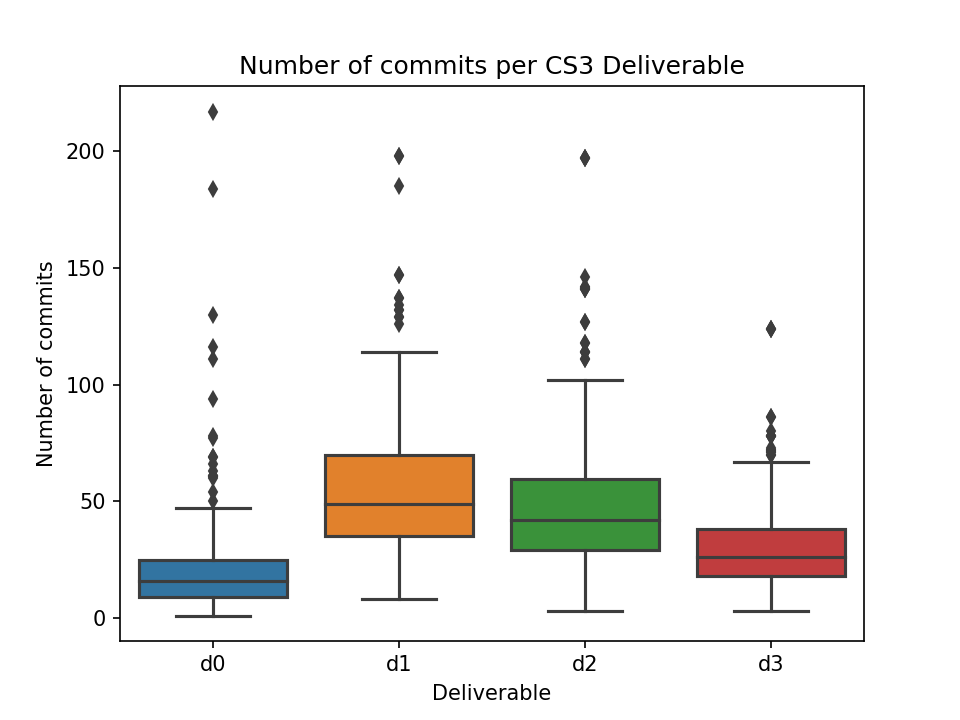
\includegraphics[width=\linewidth]{cs3-commit-boxplot.png}
\end{figure}

\begin{figure}
    \centering
    \textbf{Plot 2: Commit statistics for CS2}\par\medskip
  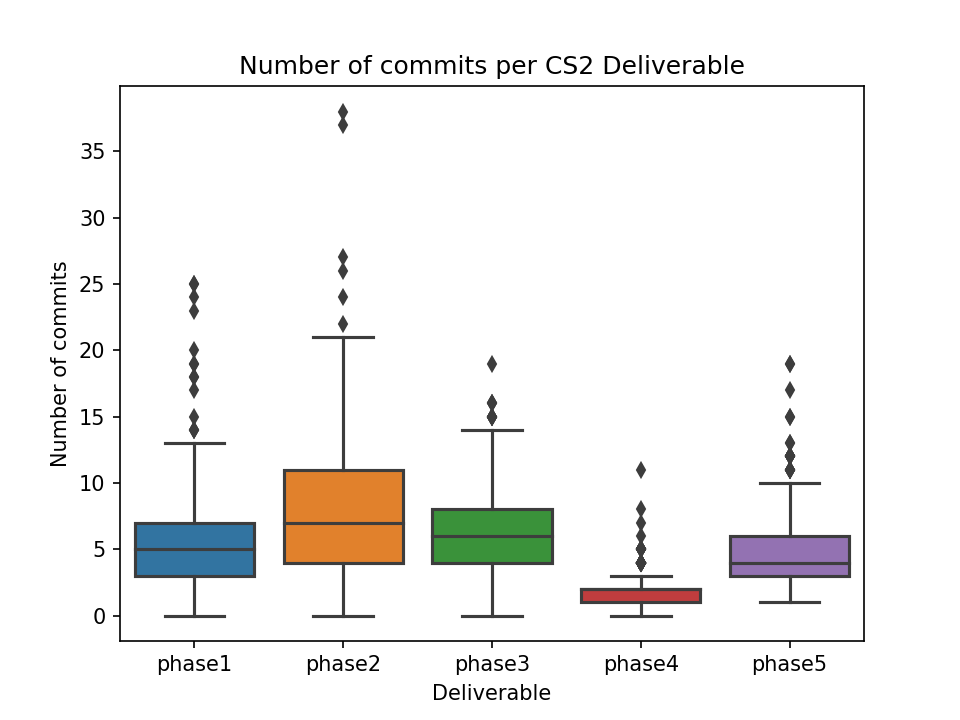
\includegraphics[width=\linewidth]{cs2-commit-boxplot.png}
\end{figure}


\section{Methods}

\subsection{Feature Selection}

A large number of features were able to be transformed from the data described in section 2. Some features which were included in the initial iterations of the classifier but were not part of the final iteration included a time until first commit, time of last commit, as well as the average number of commits per deliverable. It was observed that the number of commits in deliverable 1 had the highest predictive power (Plot 3), followed by the number of commits in deliverable 2/3, with the number of commits in deliverable 0 having the least predictive power.

\begin{figure}
    \centering
    \textbf{Plot 2: Feature Importance for CS3}\par\medskip
  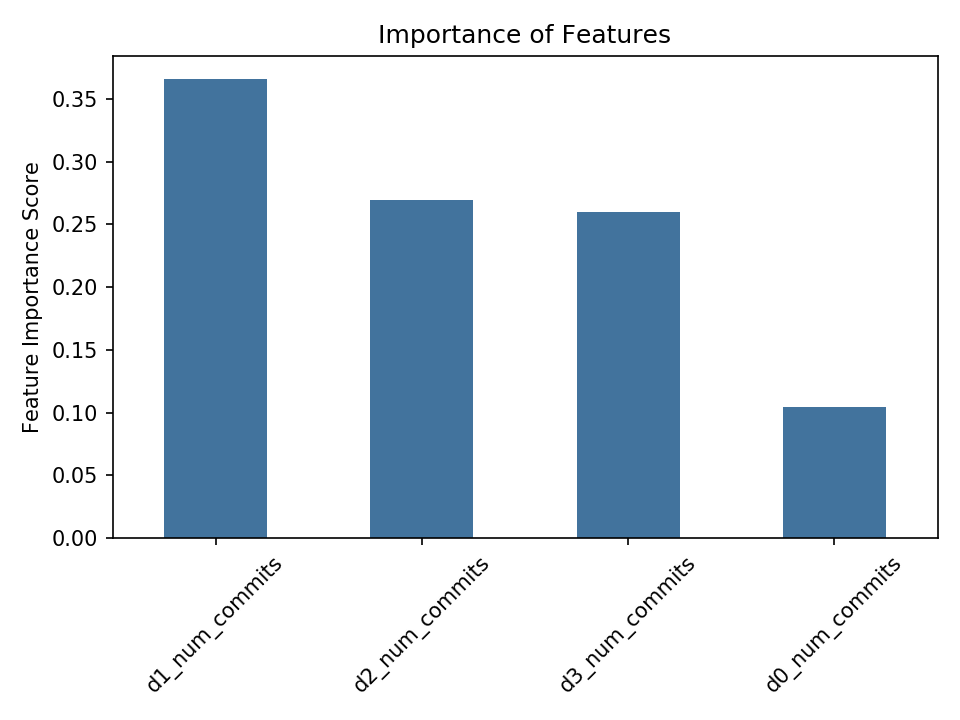
\includegraphics[width=\linewidth]{cs3-feature-importance.png}
\end{figure}

\par This describes an interesting scenario. Deliverable 0 in the CS3 course is the phase of the project which focuses entirely on students generating a set of testing suites to help validate the correctness of the code written in later phases. This may mean that the success of the student in Deliverable 0 may not be strongly correlated with their success in the entire project itself. This begs the question, are students really performing test-driven development in CS3?
\par A possible explanation for this is the fact that writing business logic and writing tests to validate business logic are two distinct skills, i.e. student proficiency in one does not necessarily imply proficiency in the other. Another explanation is the possibility that students rely more on the feedback on tests provided by AutoTest rather than their own testing suites. That being said, all 4 of the features described in (Plot 3) were used as components of the classifier.

\subsection{Classifier Production}

The Gradient Boosting Regressor (GBR) was trained and tested with a 90/10 split. This means that 90\% of the CS2 and CS3 datasets was used for training the classifier, and 10\% of the datasets were used to test the accuracy of the classifier and assign it a regression score. 

\subsection{Loss function Optimization}
The scikit-learn implementation of GBR \citestyle{scikit-learn} provides a number of loss functions that the classifier attempts to optimize. The two that I selected in training this classifier were the Huber loss and the Least Squares Loss (L2). Both the Huber and the L2 loss enabled the classifier to achieve around the same regression score. However, the L2 loss was much more stable in between each classification run. Therefore, in the final model, the L2 loss was used and optimized using regular gradient descent methods.

\subsection{Preventing Overfitting}
Overfitting was a major problem in training the classifier with a limited amount of data. In most instances of machine learning, especially in industrial applications, classifiers are trained with massive amounts of data, often with millions of examples and hundreds of features. Working with a limited amount of data from CS2 and CS3 meant that the model was especially prone to overfitting. 
\par To combat this, a 90/10 split was used during training (as previously mentioned) and the use of cross-validation was employed. 

\subsection{Results}

I was able to train a classifier with an average regression score of 0.800 (Table 1), out of a maximum score of 1.000.

\begin{table}[h]
\caption{\textbf{Gradient Boosting Regressor Performance}}
\begin{tabular}{@{}rr@{}}
\toprule
\multicolumn{1}{l}{Test Iteration} & \multicolumn{1}{l}{Regression Score} \\ \midrule
1                                  & 0.80026                              \\
2                                  & 0.80337                              \\
3                                  & 0.80319                              \\
4                                  & 0.79504                              \\ \bottomrule
\end{tabular}
\end{table}
\end{figure}

\section{Discussion}

Industrial demand for STEM graduates is the most popular it has ever been, and this is especially true for students graduating with a degree in computer science/software development. As the number of students enrolled in computer science and development courses increase to meet this demand, I expect there to be a shift toward more automated methods of student assessment. Unfortunately, this increase in automated methods could very likely come with a decrease in the human aspect of assessment, e.g. identifying students who are at risk of falling behind in the future from their current work, etc...
\par It is my hope that my classifier is the first step toward creating intelligent tools which enable educators to provide an experience usually limited to smaller class-sizes to larger, and larger classrooms. Specifically, I hope that my tool can be used to identify students before they themselves realize that they are struggling and hopefully, furnish them with the tools they need to succeed.

\section{Future work}
The classifier I present in this paper is effective when used in conjunction with a dataset which has already been collected, i.e. it uses an offline machine learning algorithm. This means that it is best used to make predictions about future events from events which have already occurred.
\par Consequently, predictions made by this classifier on real-time data, i.e. predictions on a current term based on the data collected on that term, will not be as accurate. Online machine learning \cite{1315937} methods tackle the real-time classification problem by providing algorithms to enable classifiers to make accurate predictions using data as it becomes available to them. Transforming the current classifier to use online machine learning algorithms would enable educators to use it in real-time in the courses they teach. 

\section{Acknowledgments}
This work would have not been possible without the support of a number of people. I am extremely grateful to Nick Bradley of the Software Practices Lab at the University of British Columbia who was instrumental in obtaining the data I needed to train my classifiers, and the developers of the scikit-learn machine learning library, who work tirelessly to continually lower the barrier to entry for machine learning. I also thank my friend Amy Zhu for being a source of encouragement and inspiration as I watched her perform her own directed studies. Last but not least, I thank Professor Reid Holmes, for showing me that research goes rarely as planned and for being an understanding mentor who answered more than enough questions, and entertained my possible topics, no matter how far-fetched they were. This work could not have happened without their support.


%%
%% The next two lines define the bibliography style to be used, and
%% the bibliography file.
\bibliographystyle{ACM-Reference-Format}
\bibliography{sample-base}

\end{document}
\endinput
%%
%% End of file `sample-sigchi.tex'.
